\section{Exchange Transactions}
\label{section:exchange_transactions}

% \subsection{Markets}

% One effort to explain the sustained failure or markets to equilibriate at the aggregate level is to
% try to explain failure of equilibriation as a result of the way individual economic behaviour
% aggregates to failure or otherwise of markets for single products to equilibriate, and further to
% explain failure of markets to equilibriate at the aggregate level.
% 
% A fundamental method of science and engineering is to assume as a first step, is to use the mean
% value to aggregate a collection of micro-level behaviours. Often this turns out not to be correct,
% but invariably, in virtually every system we seek to explain, there are some parts of the system we
% explain away by averaging out noisy behaviour. 
% 
% If we use the same technique for understanding economic behaviour, we would, as a first step assume
% that we can average markets for single goods or services, result in an aggregate supply or demand
% close to zero.
% 
% If we use the same technique for understanding economic behaviour, we would, as a first step assume
% that we can aggregate our model of supply and demand for single goods or services, and arrive at a
% aggregate where aggregate supply or demand is close to zero.
% 
% Since this conclusion is contrary to facts, economists have directed their efforts at modifying the
% supply and demand model in many ways in an effort to explain this contradiction between fact and
% theory.
% 
% What is clear, however, is that the explanation has to be sufficiently fundamental to explain the
% remarkably consistent fact of excess aggregate supply and the rarity of aggregate market
% equilibrium. As put forward by Lucas, economists have yet to find a convincing understanding of
% this fact, let alone to find a solution to the problem of equilibrium failure or the problem of
% a sustained positive unemployment rate. 
% 
% Since our explanation of these facts is outside is not a part of the supply and demand model, we
% assume our simplest model of market behaviour, and that markets at the aggregate level do in fact
% equilibriate, relying on the law of large averages.

\subsection{An Exchange Transaction Only Model}

We will start with a model simplified from Figure \ref{fig:economic_feedback_schema1}. that includes only
exchange transactions.

\begin{figure}[H]
\centering
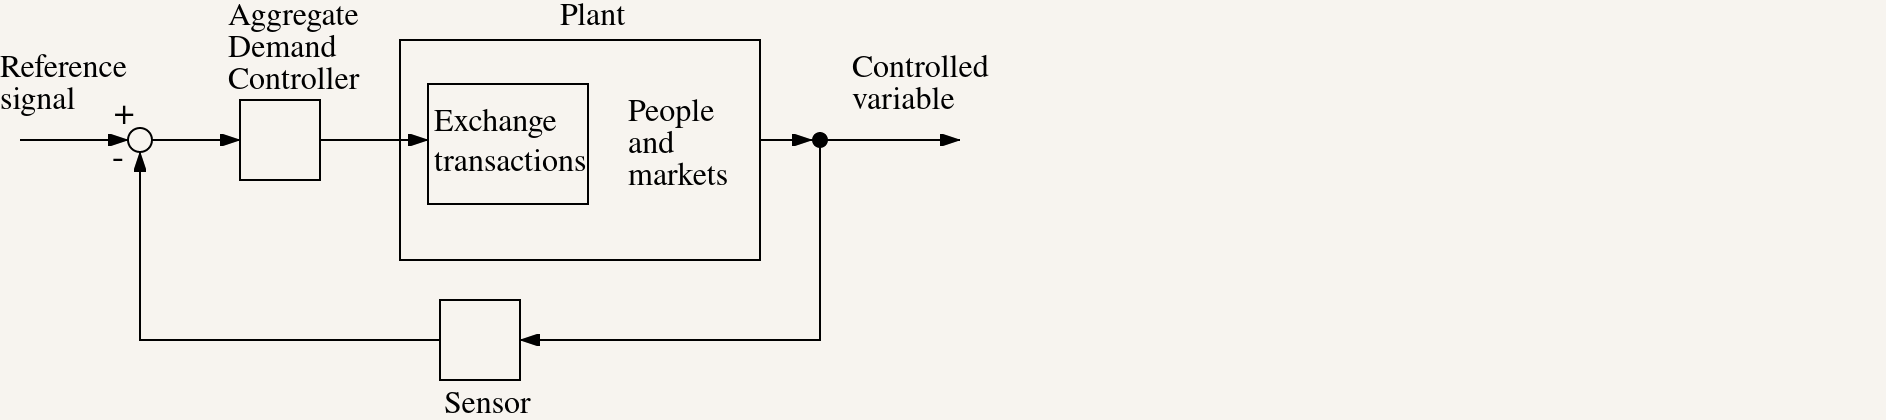
\includegraphics[scale=0.60]{03_exchange_transactions/png/exchange_only_feedback_schema}
\caption{Exchange Only Feedback Schema}
\label{fig:exchange_only_feedback_schema1}
\end{figure}

\subsection{Price and Quantity}

\subsection{Control of Price Level}

Before examining exchange transactions, we will briefly consider the feedback control mechanism.
Indexation is an important method for controlling distributed systems like a currency. An index is a
single value that is utilized by multiple components. An example of indexation in digital currencies
is Bitcoin's method for regulating the rate of production of blocks by Bitcoin miners. In this case
the indexation is algorithmic rather than controlled by a central authority. TODO

Another example of indexation is 

The simplest way to control the price level in a digital currency is to use indexation.





[TODO]

The feedback control loop does not work, however, in legacy currencies because the core currency
doesn't account for all money. Most money in legacy currencies is banking money, termed M1, M2 and
M3. Under these conditions, money authorities must use alternative methods to try and induce
financial institutions to increase the amount of banking money mainly through changing the interest
rate at which the money authority lends core currency to those financial institutions. At times this
method has been effective at controlling the price level, at other times less so. The process lacks
precision and has a long time-lag, making its use as the main mechanism for controlling economic
conditions problematic. Its effectiveness is also determined by financial institution's ability and
willingness to respond to decreases or increases in the monetary authority's core lending rate in a
way the maps to increases or decreases in aggregate demand.

\subsection{Market Symmetry}
